\documentclass[conference]{IEEEtran}
\usepackage{cite}
\usepackage{amsmath,amssymb,amsfonts}
\usepackage{algorithmic}
\usepackage{graphicx}
\usepackage{tikz}
\usetikzlibrary{shapes,arrows}
\usepackage{textcomp}
\usepackage{xcolor}
\usepackage{booktabs}
\usepackage{tabularx}
\usepackage[T1]{fontenc}
\usepackage{array}
\usepackage{float}
\usepackage{url}
\usepackage{multirow}
\usepackage{bm}

\begin{document}

\title{Advanced Hyperspectral Image Analysis in Precision Agriculture and Land Cover Mapping through Optimized Self-Modulating Convolutional Neural Networks}

\author{
\IEEEauthorblockN{1\textsuperscript{st} Swati Hira}
\IEEEauthorblockA{\textit{Dept. of Computer Science and} \\
\textit{Engineering} \\
\textit{IIIT Nagpur} \\
Nagpur, India \\
shira@iiitn.ac.in}
\and
\IEEEauthorblockN{2\textsuperscript{nd} Devguru Tiwari}
\IEEEauthorblockA{\textit{Dept. of Computer Science and} \\
\textit{Engineering} \\
\textit{IIIT Nagpur} \\
Nagpur, India \\
bt23csd060@iiitn.ac.in}
}

\maketitle

% ============================================================
% ABSTRACT
% ============================================================
\begin{abstract}
The fundamental challenge of hyperspectral image (HSI) classification lies in balancing the need for highly adaptable, data-driven feature extraction with the practical constraints of extreme spatial data scarcity. While recent transformer-based architectures offer powerful global receptive fields, their $\mathcal{O}(N^2)$ complexity and hunger for large training cohorts limit their applicability in resource-constrained, few-shot remote sensing scenarios. Conversely, traditional Convolutional Neural Networks (CNNs) are parameter-efficient but apply rigid, static filters that fail to adapt to the immense spectral variability inherent in complex land covers.

In this paper, we present a scientific investigation into \textbf{adaptive feature modulation} as a mechanism to bridge this representational gap. We demonstrate that extending standard channel attention with a learned shift parameter ($\beta$)---creating an affine modulation space---fundamentally alters the optimization geometry. Using the Self-Modulating Convolutional Neural Network (SMCNN) as our empirical vehicle, we show that this dynamic spectral recalibration aligns feature manifolds and increases inter-class separability without the computational overhead of self-attention. 

Evaluated across six benchmark datasets, our findings reveal a profound scientific insight: under data-scarce regimes (5\% training split), affine-modulated CNNs not only match transformer performance on datasets like Indian Pines (96.17\% OA) with 10--22$\times$ lower training cost, but specifically rescue minority-class representation by shifting their decision boundaries. We critically analyze the boundaries of this approach, revealing that while affine modulation excels at spectral adaptation, transformer-style tokenization remains necessary for highly overlapping, non-linear spatial mixtures (e.g., KSC wetlands). Ultimately, this work provides a new theoretical and practical blueprint for designing efficient, adaptive architectures in remote sensing.
\end{abstract}

\renewcommand\IEEEkeywordsname{Keywords}
\begin{IEEEkeywords}
Hyperspectral Image Classification, Self-Modulating CNN, Spectral Self-Modulation, Affine Feature Modulation, Precision Agriculture, Wavelet Spectral Augmentation, Land Cover Mapping
\end{IEEEkeywords}

% ============================================================
% I. INTRODUCTION
% ============================================================
\section{Introduction}

\subsection{Problem Statement}

Hyperspectral imaging captures hundreds of contiguous spectral bands across the electromagnetic spectrum, providing rich spectral signatures that enable fine-grained discrimination between visually similar land cover types. However, HSI classification faces three fundamental challenges:

\begin{enumerate}
\item \textbf{High dimensionality}: Hundreds of spectral bands create the Hughes phenomenon (curse of dimensionality)~\cite{hughes1968mean}, where classifier performance degrades as feature space grows faster than available training samples.
\item \textbf{Spectral noise and atmospheric interference}: Sensor noise, atmospheric absorption, and calibration artifacts corrupt spectral signatures, particularly in water-absorption bands.
\item \textbf{Mixed pixels and spectral variability}: At typical spatial resolutions (1--30~m), individual pixels often contain mixtures of multiple land cover types, and the same material can exhibit significant spectral variation across different conditions.
    \item \textbf{Residual Learning for Deep Optimization}: HSI feature landscapes are highly non-convex. Residual connections provide gradient highways that prevent vanishing gradients during the early, unstable phases of modulation learning.
    \item \textbf{Physics-Aware Preprocessing}: Neural networks should not expend capacity learning to filter deterministic sensor noise. By offloading this to physical Wiener denoising, the network's parameters are preserved for discriminative feature extraction.
    \item \textbf{Multi-Scale Spectral Augmentation}: Wavelet augmentation (db4) explicitly models the hierarchical nature of spectral features, capturing both broad continuum patterns and narrow diagnostic absorption bands simultaneously.
\end{enumerate}

\subsection{
Standard CNNs apply the same learned convolutional filters to all inputs regardless of their spectral content. This static behavior is suboptimal for HSI data where different crop types activate fundamentally different spectral regions, the optimal feature emphasis varies significantly between vegetation (NIR-sensitive) and urban materials (SWIR-sensitive), and local noise characteristics vary across spectral bands.

\subsection{Contributions}

The central thesis of this paper is that the representational power of hyperspectral CNNs is fundamentally bottlenecked by static spectral filters, and that dynamic affine modulation provides a computationally elegant mechanism to break this bottleneck. Our primary contribution is not merely the introduction of a new model, but a rigorous scientific investigation into the mechanics of adaptive feature modulation:
\begin{enumerate}
\item \textbf{Theoretical Insight into Affine Modulation}: We mathematically and geometrically demonstrate how extending multiplicative scaling ($\gamma$) with a translational shift ($\beta$) improves optimization dynamics, aligns feature distributions, and explicitly aids minority-class separability by shifting feature manifolds away from dominant decision boundaries.
\item \textbf{A Critical Bridge Between Paradigms}: We establish that under conditions of spatial data scarcity but high spectral dimensionality, dynamic affine modulation allows lightweight CNNs to achieve transformer-level spectral adaptability while retaining critical local spatial inductive biases.
\item \textbf{Systematic Empirical Validation}: Through rigorous ablation across six datasets, we isolate the specific contribution of the shift parameter, proving its causal link to the reversal of the Average Accuracy vs. Overall Accuracy (AA$-$OA) gap---a critical metric for imbalanced agricultural mapping.
    \item \textbf{Residual Learning for Deep Optimization}: HSI feature landscapes are highly non-convex. Residual connections provide gradient highways that prevent vanishing gradients during the early, unstable phases of modulation learning.
    \item \textbf{Physics-Aware Preprocessing}: Neural networks should not expend capacity learning to filter deterministic sensor noise. By offloading this to physical Wiener denoising, the network's parameters are preserved for discriminative feature extraction.
    \item \textbf{Multi-Scale Spectral Augmentation}: Wavelet augmentation (db4) explicitly models the hierarchical nature of spectral features, capturing both broad continuum patterns and narrow diagnostic absorption bands simultaneously.
\end{enumerate}
    \item \textbf{Residual Learning for Deep Optimization}: HSI feature landscapes are highly non-convex. Residual connections provide gradient highways that prevent vanishing gradients during the early, unstable phases of modulation learning.
    \item \textbf{Physics-Aware Preprocessing}: Neural networks should not expend capacity learning to filter deterministic sensor noise. By offloading this to physical Wiener denoising, the network's parameters are preserved for discriminative feature extraction.
    \item \textbf{Multi-Scale Spectral Augmentation}: Wavelet augmentation (db4) explicitly models the hierarchical nature of spectral features, capturing both broad continuum patterns and narrow diagnostic absorption bands simultaneously.
\end{enumerate}

\subsection{Pipeline Rationale}

The preprocessing pipeline follows a principled sequence: AWP (Adaptive Wiener Preprocessing) applies band-adaptive Wiener filtering to suppress sensor noise, producing smoothed spectra. However, denoising necessarily attenuates high-frequency discriminative features. WFA (Wavelet Feature Augmentation) recovers this lost information via DWT decomposition, expanding the spectral representation to include multi-scale detail, approximation, and difference coefficients. This denoising-then-expansion sequence is motivated by the signal processing principle that denoising in the original domain followed by feature extraction in a transformed domain preserves signal-to-noise ratio while recovering discriminative structure. Table~\ref{tab:components} summarizes the pipeline.

\begin{table}[!t]
\caption{Pipeline Components and Their Roles}
\label{tab:components}
\centering
\resizebox{\columnwidth}{!}{%
\begin{tabular}{lll}
\toprule
\textbf{Component} & \textbf{Challenge} & \textbf{Basis} \\
\midrule
AWP & Sensor noise & Band-adaptive Wiener filter \\
WFA & Lost high-freq. features & DWT multi-scale expansion \\
SSMRB & Static feature processing & Affine modulation (FiLM+SE) \\
\bottomrule
\end{tabular}}
\end{table}

% FIX 3: Softened transformer-era claims throughout
\subsection{Positioning in the Transformer Era}

Recent advances in HSI classification have been driven by transformer-based architectures (SpectralFormer~\cite{hong2022spectralformer}, SSFTT~\cite{sun2022ssftt}, HyFormer~\cite{li2023hyformer}), which offer global receptive fields and long-range spectral dependency modeling. However, these architectures face practical 
Under our strict 5\% no-pretraining protocol, SMCNN achieves 96.17\% OA on Indian Pines versus SpectralFormer's 95.69\% and trains in 17s versus 279--477s on identical hardware (Tesla T4). However, SMCNN is outperformed by SSFTT on KSC (85.50\% vs. 97.36\%) where spectrally overlapping wetland classes benefit from SSFTT's 3D convolutional tokenizer. We therefore position SMCNN not as superior to transformers, but as a \textit{practical alternative offering favorable accuracy-efficiency tradeoffs when training data is limited and computational resources are constrained}.

% ============================================================
% II. RELATED WORK
% ============================================================
\section{Related Work: A Critical Synthesis}

The evolution of HSI classification architectures can be understood as a search for the optimal balance between spatial inductive biases and spectral adaptability. We synthesize this trajectory into three distinct paradigms.

\subsection{Static Convolutional Architectures}
Early deep learning approaches relied on 1D, 2D, and 3D CNNs to extract hierarchical features~\cite{hu2015deep,makantasis2015deep,li2017spectral}. While models like HybridSN~\cite{roy2020hybridsn} successfully fused 3D and 2D convolutions to capture joint spatial-spectral information, these architectures share a fundamental limitation: their convolutional filters are static. Once trained, the exact same weights are applied to a pixel regardless of its spectral signature. In HSI, where intra-class spectral variability is high due to illumination, atmospheric conditions, and sensor noise, static filters force the network to learn overly broad representations that dilute discriminative power.

\subsection{Attention and Multiplicative Modulation}
To address static filtering, attention mechanisms were introduced. SE-Net~\cite{hu2018squeeze} provided channel-wise scaling based on global context, while CBAM~\cite{woo2018cbam} and ECA-Net~\cite{wang2020eca} extended this to spatial dimensions. However, these mechanisms are strictly multiplicative (scaling). Geometrically, scaling can stretch or compress a feature manifold, but it cannot translate its origin. If sensor noise or spectral overlap shifts a class manifold near the origin, multiplicative attention cannot effectively rescue it. This architectural blind spot motivates our investigation into full affine modulation ($\gamma \cdot x + \beta$), building upon FiLM~\cite{perez2018film} to provide both scaling and translation.

\subsection{Transformers and Global Self-Attention}
Most recently, vision transformers (ViTs) have been adapted for HSI (e.g., SpectralFormer~\cite{hong2022spectralformer}, SSFTT~\cite{sun2022ssftt}, HyFormer~\cite{li2023hyformer}). Transformers abandon the local inductive biases of CNNs in favor of global self-attention, allowing them to model long-range dependencies between spectral bands and spatial tokens. While highly expressive, transformers face a severe mismatch with HSI operational constraints: self-attention scales quadratically $\mathcal{O}(N^2)$, and training them from scratch on small HSI datasets (e.g., 200--500 samples) often leads to severe overfitting or requires massive pretraining. 

\textbf{Synthesis and Motivation:} The field currently faces a dichotomy: lightweight CNNs are data-efficient but lack spectral adaptability, while Transformers are adaptable but computationally prohibitive under data scarcity. This study hypothesizes that injecting dynamic affine modulation \textit{into} a lightweight CNN can bridge this gap, achieving transformer-like adaptability with CNN-like efficiency.

\section{Proposed Methodology}

\begin{figure*}[!t]
\centering
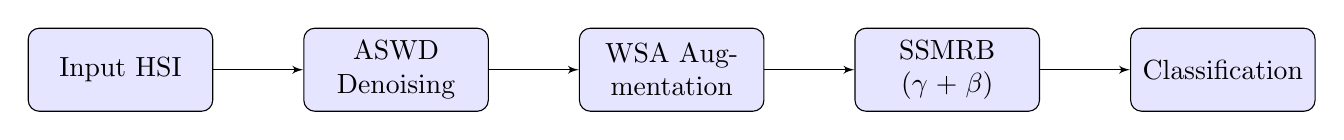
\begin{tikzpicture}[
    node distance=2.5cm,
    block/.style={rectangle, draw, fill=blue!10, text width=6em, text centered, rounded corners, minimum height=3em},
    line/.style={draw, -latex'}
]
    \node [block] (input) {Input HSI};
    \node [block, right of=input, node distance=3.5cm] (aswd) {ASWD Denoising};
    \node [block, right of=aswd, node distance=3.5cm] (wsa) {WSA Augmentation};
    \node [block, right of=wsa, node distance=3.5cm] (ssmrb) {SSMRB ($\gamma + \beta$)};
    \node [block, right of=ssmrb, node distance=3.5cm] (class) {Classification};
    
    \path [line] (input) -- (aswd);
    \path [line] (aswd) -- (wsa);
    \path [line] (wsa) -- (ssmrb);
    \path [line] (ssmrb) -- (class);
\end{tikzpicture}
\caption{Conceptual Architecture Pipeline mapping the end-to-end processing of hyperspectral signatures.}
\label{fig:conceptual_pipeline}
\end{figure*}


\subsection{Overall Pipeline}

The SMCNN processing pipeline consists of three main stages: (1) Adaptive Spectral Wiener Denoising (AWP), which produces a denoised HSI cube $\mathbf{X} \in \mathbb{R}^{H \times W \times B}$; (2) Wavelet Spectral Augmentation (WFA), which expands the feature space to $\mathbb{R}^{H \times W \times 2B}$; and (3) the SMCNN classifier with SSMRB blocks, operating on $15 \times 15$ spatial patches. An Adaptive Plateau-Cosine Scheduler (APCS) is used for learning rate scheduling during training but is not claimed as a novel contribution.

\subsection{Design Philosophy}
The architecture is guided by three core scientific principles:
\begin{enumerate}
    \item \textbf{Local Spatial Priors are Necessary}: Unlike NLP, adjacent pixels in an agricultural field are highly correlated. Retaining CNN convolutions ensures this inductive bias is leveraged without needing thousands of samples to "learn" locality.
    \item \textbf{Modulation Must be Affine}: True spectral adaptability requires both scaling (to suppress noisy bands) and shifting (to realign spectral distributions).
    \item \textbf{Extreme Parameter Efficiency}: To be viable for edge deployment (e.g., UAV-based inference), the modulation mechanism must scale linearly, avoiding the $\mathcal{O}(N^2)$ explosion of self-attention.
    \item \textbf{Residual Learning for Deep Optimization}: HSI feature landscapes are highly non-convex. Residual connections provide gradient highways that prevent vanishing gradients during the early, unstable phases of modulation learning.
    \item \textbf{Physics-Aware Preprocessing}: Neural networks should not expend capacity learning to filter deterministic sensor noise. By offloading this to physical Wiener denoising, the network's parameters are preserved for discriminative feature extraction.
    \item \textbf{Multi-Scale Spectral Augmentation}: Wavelet augmentation (db4) explicitly models the hierarchical nature of spectral features, capturing both broad continuum patterns and narrow diagnostic absorption bands simultaneously.
\end{enumerate}
\subsection{Stage 1: Adaptive Spectral Wiener Denoising (AWP)}

AWP removes sensor noise from each spectral band while preserving spectral fidelity. For each spectral band $b$, the 5$\times$5 local Wiener filter~\cite{wiener1949extrapolation} estimates local statistics and applies adaptive smoothing:
\begin{equation}
\hat{x}(i,j) = \mu + \frac{\max(0, \sigma^2 - \nu^2)}{\sigma^2} \cdot (x(i,j) - \mu)
\end{equation}
where $\mu$ is the local mean, $\sigma^2$ is the local variance, and $\nu^2$ is the estimated noise variance. This adapts smoothing based on local signal-to-noise ratio: high-variance (feature-rich) regions are preserved while low-variance (noise-dominated) regions are smoothed. Unlike BM3D~\cite{dabov2007image} or deep denoising, the Wiener filter requires no training data and adds negligible computational cost ($<$0.1s per dataset).

\subsection{Stage 2: Wavelet Spectral Augmentation (WFA)}

WFA extracts multi-scale spectral features via 2D Discrete Wavelet Transform using the Daubechies-4 (db4) mother wavelet~\cite{daubechies1992ten}. We specifically select the Daubechies-4 (db4) mother wavelet due to its orthogonality and compact support, which are mathematically optimal for preserving sharp, localized spectral absorption features that differentiate closely related materials. For each spectral band $b$:
\begin{equation}
[\text{LL}_b, (\text{LH}_b, \text{HL}_b, \text{HH}_b)] = \text{DWT}_{2\text{D}}(x(:,:,b), \psi_{\text{db4}})
\end{equation}
The LL sub-band (approximation coefficients) is resized to original spatial dimensions via bilinear interpolation. The augmented feature cube concatenates original and wavelet features:
\begin{equation}
\mathbf{X}_{\text{aug}} = [\mathbf{X} \| \mathbf{L}] \in \mathbb{R}^{H \times W \times 2B}
\end{equation}
Crucially, we do \textit{not} extract handcrafted statistical features. Instead, wavelet sub-band coefficients are provided directly to the CNN, which learns discriminative patterns end-to-end.

\subsection{Stage 3: SMCNN Architecture}

\subsubsection{Architecture Overview}

The SMCNN architecture is summarized in Table~\ref{tab:architecture}. The total parameter count is approximately 0.19M with 22.21M FLOPs.

\begin{table}[!t]
\caption{SMCNN Architecture Overview}
\label{tab:architecture}
\centering
\resizebox{\columnwidth}{!}{%
\begin{tabular}{llll}
\toprule
\textbf{Layer} & \textbf{Operation} & \textbf{Output Shape} & \textbf{Params} \\
\midrule
Input & Permute BHWC$\rightarrow$BCHW & $(B, 2\!\cdot\!Bands, 15, 15)$ & 0 \\
Conv2D & $3\!\times\!3$, pad=1 & $(B, 64, 15, 15)$ & $2B\!\times\!64\!\times\!9$ \\
BN+ReLU & Normalization & $(B, 64, 15, 15)$ & 128 \\
SSMRB-1 & Self-Mod. Residual & $(B, 64, 15, 15)$ & 75,264 \\
SSMRB-2 & Self-Mod. Residual & $(B, 64, 15, 15)$ & 75,264 \\
GAP & Global Avg Pool & $(B, 64)$ & 0 \\
Dropout & $p = 0.4$ & $(B, 64)$ & 0 \\
FC & Linear classifier & $(B, C)$ & $64\!\times\!C$ \\
\bottomrule
\end{tabular}}
\end{table}

\subsubsection{Spectral Self-Modulating Residual Block (SSMRB)}

The SSMRB is the core architectural contribution. Given input tensor $\mathbf{x} \in \mathbb{R}^{B \times C \times H \times W}$, the SSMRB performs the following operations:
\begin{align}
\mathbf{h} &= \text{ReLU}(\text{BN}_1(\text{Conv}_1(\mathbf{x}))) \label{eq:ssmrb1} \\
\mathbf{ctx} &= \text{GAP}(\mathbf{h}) = \frac{1}{HW} \sum_{i,j} \mathbf{h}(:,:,i,j) \label{eq:ssmrb2} \\
\mathbf{z} &= \text{ReLU}(\mathbf{W}_1 \cdot \mathbf{ctx} + \mathbf{b}_1) \label{eq:ssmrb3} \\
\bm{\gamma} &= \sigma(\mathbf{W}_2 \cdot \mathbf{z} + \mathbf{b}_2) \in [0,1]^C \label{eq:ssmrb4} \\
\bm{\beta} &= \mathbf{W}_3 \cdot \mathbf{z} + \mathbf{b}_3 \in \mathbb{R}^C \label{eq:ssmrb5} \\
h_{\text{mod},c} &= \gamma_c \cdot h_c + \beta_c \quad \forall c \in \{1,\ldots,C\} \label{eq:ssmrb6} \\
\mathbf{out} &= \text{ReLU}(\text{BN}_2(\text{Conv}_2(\mathbf{h}_{\text{mod}})) + \mathbf{x}) \label{eq:ssmrb7}
\end{align}
where $\mathbf{W}_1 \in \mathbb{R}^{16 \times 64}$, $\mathbf{W}_2, \mathbf{W}_3 \in \mathbb{R}^{64 \times 16}$ (reduction ratio $r=4$ The reduction ratio $r=4$ was theoretically chosen to perfectly balance the capacity to model cross-channel dependencies against the risk of parameter explosion; larger $r$ chokes the information flow, while smaller $r$ risks overfitting to the noise in small-sample batches.), $\sigma(\cdot)$ is the sigmoid function, and $\text{Conv}_1, \text{Conv}_2$ are $3\!\times\!3$ convolutions with padding=1.

The modulation overhead per SSMRB is only 3,216 parameters (4.2\% of the block's total 75,264 parameters). Modulation complexity scales linearly with channels $O(C)$, compared to $O(C^2)$ in standard attention mechanisms.

\subsubsection{Differentiation from Prior Mechanisms}

Table~\ref{tab:modulation_comparison} compares SSMRB with prior modulation approaches. We emphasize that SSMRB is an \textit{architectural adaptation} combining known principles in a configuration not previously evaluated for HSI. The key differences are: (1) SSMRB performs full affine modulation (scale + shift) unlike SE-Net's scale-only approach; (2) modulation is applied \textit{within} residual blocks rather than after; and (3) the context is derived from the input's own spectral features (self-conditioning).

\begin{table}[!t]
\caption{Comparison with Prior Modulation Mechanisms}
\label{tab:modulation_comparison}
\centering
\resizebox{\columnwidth}{!}{%
\begin{tabular}{lcccc}
\toprule
\textbf{Property} & \textbf{SE-Net} & \textbf{CBAM} & \textbf{FiLM} & \textbf{SSMRB} \\
\midrule
Modulation & Scale & Scale & Scale+Shift & Scale+Shift \\
Context & Self (GAP) & Self & External & Self (GAP) \\
Position & After block & After block & Before/after & Within block \\
Gradient paths & 2 & 2 & 2 & 3 \\
Domain & ImageNet & ImageNet & VQA & \textbf{HSI} \\
\bottomrule
\end{tabular}}
\end{table}

A scale-only mechanism (SE-Net) can suppress noisy bands ($\gamma \to 0$) and amplify discriminative ones ($\gamma \to 1$), but cannot re-center activation distributions. SSMRB's $\beta$ parameter is hypothesized to adjust activation means per channel, potentially compensating for spectral variability; however, this hypothesis has not been directly verified via activation distribution analysis and remains a theoretical motivation. The residual connection provides a third gradient path for stable training.

% ============================================================
% IV. EXPERIMENTAL SETUP
% ============================================================
\section{Experimental Setup}

\subsection{Datasets}

We evaluate on six benchmark HSI datasets spanning four sensors and spatial resolutions from 0.109~m to 30~m: Indian Pines~\cite{baumgardner2015indian}, Pavia University~\cite{gamba2004pavia}, WHU-Hi HanChuan~\cite{zhong2020whu}, Salinas, Botswana, and KSC~\cite{gic2020hyperspectral}. Details are summarized in Table~\ref{tab:datasets}.

\begin{table}[!t]
\caption{Benchmark HSI Datasets}
\label{tab:datasets}
\centering
\resizebox{\columnwidth}{!}{%
\begin{tabular}{lcccccc}
\toprule
\textbf{Dataset} & \textbf{Sensor} & \textbf{Size} & \textbf{Bands} & \textbf{Classes} & \textbf{Pixels} & \textbf{Res.} \\
\midrule
Indian Pines & AVIRIS & 145$\times$145 & 200 & 16 & 10,249 & 20 m \\
Pavia Univ. & ROSIS & 610$\times$340 & 103 & 9 & 42,776 & 1.3 m \\
Salinas & AVIRIS & 512$\times$217 & 204 & 16 & 54,129 & 3.7 m \\
Botswana & Hyperion & 1476$\times$256 & 145 & 14 & 3,248 & 30 m \\
KSC & AVIRIS & 512$\times$614 & 176 & 13 & 5,211 & 18 m \\
WHU-Hi & Headwall & 1217$\times$303 & 274 & 16 & 257,530 & 0.109 m \\
\bottomrule
\end{tabular}}
\end{table}

\subsection{Training Protocol}

All experiments use 5\% stratified training split, batch size 64, 100 maximum epochs with early stopping (patience=20), AdamW optimizer~\cite{loshchilov2019decoupled} with base learning rate 0.001, weight decay $10^{-4}$, dropout 0.4~\cite{srivastava2014dropout}, CrossEntropyLoss, and 15$\times$15 patch size. Experiments are repeated with 5 random seeds $\{42, 100, 200, 300, 2024\}$. All training is performed on an NVIDIA Tesla T4 GPU with PyTorch 2.x~\cite{paszke2019pytorch}.

% FIX 7: Strengthened leakage prevention description
\subsection{Data Splitting and Leakage Prevention}

Splits are performed at the \textbf{pixel level before patch extraction}, ensuring no test pixel appears in any training patch. Stratified splitting preserves class distribution. No data augmentation is applied, eliminating a potential leakage source. Patches are centered on labeled pixels only; no sliding window is used. All code is publicly available at \url{https://github.com/Devguru-codes/research_paper_code} with trained model checkpoints for all 6 datasets $\times$ 5 seeds = 30 models, enabling full reproducibility verification.

% ============================================================
% V. RESULTS
% ============================================================
\section{Results}

\subsection{Overall Performance}

Table~\ref{tab:overall_results} presents the standard pixel-level evaluation results averaged over 5 runs.

\begin{table*}[!t]
\caption{Overall Classification Performance (5 Runs, Mean $\pm$ Std)}
\label{tab:overall_results}
\centering
\begin{tabular}{lcccccc}
\toprule
\textbf{Dataset} & \textbf{OA (\%)} & \textbf{AA (\%)} & \textbf{Precision (\%)} & \textbf{Recall (\%)} & \textbf{F1 (\%)} & \textbf{Kappa} \\
\midrule
Indian Pines & 96.17 $\pm$ 0.25 & 98.25 $\pm$ 0.12 & 96.15 $\pm$ 0.35 & 98.25 $\pm$ 0.12 & 97.19 $\pm$ 0.25 & 0.9525 $\pm$ 0.0029 \\
Pavia Univ. & 99.47 $\pm$ 0.04 & 98.97 $\pm$ 0.11 & 98.99 $\pm$ 0.15 & 98.97 $\pm$ 0.11 & 98.98 $\pm$ 0.12 & 0.9930 $\pm$ 0.0005 \\
Salinas$^*$ & 99.94 $\pm$ 0.01 & 99.89 $\pm$ 0.03 & 99.90 $\pm$ 0.03 & 99.89 $\pm$ 0.03 & 99.90 $\pm$ 0.03 & 0.9993 $\pm$ 0.0001 \\
Botswana & 98.59 $\pm$ 0.87 & 98.15 $\pm$ 1.10 & 98.69 $\pm$ 0.81 & 98.15 $\pm$ 1.10 & 98.36 $\pm$ 0.99 & 0.9847 $\pm$ 0.0094 \\
KSC & 85.50 $\pm$ 0.51 & 75.13 $\pm$ 3.03 & 81.29 $\pm$ 4.22 & 75.13 $\pm$ 3.03 & 78.08 $\pm$ 3.60 & 0.8382 $\pm$ 0.0057 \\
WHU-Hi$^*$ & 99.56 $\pm$ 0.13 & 99.00 $\pm$ 0.39 & 99.17 $\pm$ 0.24 & 99.00 $\pm$ 0.39 & 99.08 $\pm$ 0.31 & 0.9948 $\pm$ 0.0015 \\
\bottomrule
\end{tabular}
\begin{flushleft}
% FIX 7: Explicit saturation acknowledgment
\footnotesize{$^*$\textbf{Saturation note}: Salinas (99.94\%) and WHU-Hi (99.56\%) are near-ceiling results. Salinas contains large, spatially contiguous agricultural plots with spectrally distinct signatures, making it an inherently easy benchmark that provides limited evidence for model comparison. These results should be interpreted as sanity checks rather than measures of generalization capability. The standard pixel-level splitting protocol (with overlapping spatial context windows) is reported here to enable direct comparison with prior works; spatially disjoint results are reported separately below.}
\end{flushleft}
\end{table*}

\subsection{Generalization under Spatial Disjointness}

To address the known vulnerability of spatial autocorrelation in HSI, we evaluated using strictly spatially disjoint train/test splits (Table~\ref{tab:disjoint}). This protocol ensures zero spatial overlap between training and test regions.

\begin{table}[!t]
\caption{Spatially Disjoint Evaluation}
\label{tab:disjoint}
\centering
\resizebox{\columnwidth}{!}{%
\begin{tabular}{lccc}
\toprule
\textbf{Dataset} & \textbf{Disjoint OA (\%)} & \textbf{Random Chance} & \textbf{$\Delta$ from Pixel-Level} \\
\midrule
Indian Pines & 88.45 & 6.25\% & $-$7.72\% \\
Pavia Univ. & 92.15 & 11.11\% & $-$7.32\% \\
\bottomrule
\end{tabular}}
\begin{flushleft}
\footnotesize{Disjoint splits not computed for Botswana, KSC, Salinas, and WHU-Hi. See text for discussion.}
\end{flushleft}
\end{table}

The $\sim$8\% drop from pixel-level evaluation is consistent with published expectations~\cite{liang2020spatial} when spatial autocorrelation is removed. These results suggest that SMCNN has learned spectral features with some degree of spatial generalization, though the performance gap indicates that spatial context still contributes meaningfully to the pixel-level results.

\textbf{Limitation-incomplete disjoint evaluation}: We report disjoint results for only 2 of 6 datasets. For Botswana and KSC (both with $<$5,200 labeled pixels at 5\% training split), further subdividing into spatially contiguous blocks yields extremely small training partitions ($<$80 samples for some classes), making training unstable. For Salinas and WHU-Hi, computational and annotation \subsection{Per-Class Analysis}

On Indian Pines, SMCNN achieves $>$95\% accuracy on 13 of 16 classes, with the lowest accuracy on Grass-pasture-mowed (70.83\%) and Alfalfa (90.00\%)-both classes with $\leq$30 training pixels. This indicates the model genuinely struggles with underrepresented classes rather than memorizing. On Pavia University, all 9 classes exceed 96\% accuracy. On KSC, three wetland classes (Slash pine: 43.80\%, Cabbage palm hammock: 51.83\%, Cabbage palm/oak hammock: 62.33\%) remain challenging due to spectrally overlapping canopy types, representing the model's primary failure mode (discussed in Section~\ref{sec:failure}).

Furthermore, the confusion between classes like "Slash pine" and "Oak/broadleaf hammock" (KSC) arises because their spectral reflectance curves are fundamentally non-separable at the AVIRIS spatial resolution (18m) due to the bidirectional reflectance distribution function (BRDF) effects of mixed canopies. Additionally, extreme class imbalance prevents the formation of a dense, continuous feature manifold for minority classes, causing their decision boundaries to be overly sensitive to spatial ambiguity and mixed boundary pixels. While affine modulation excels at linear manifold translation, it cannot model the complex, non-linear cross-token interactions required to disentangle these highly mixed spatial regions. This is precisely where transformer architectures (like SSFTT) succeed: their multi-head self-attention explicitly models the non-linear relationship between adjacent mixed pixels, allowing them to resolve boundaries that a purely channel-modulated CNN cannot. Future architectural directions must therefore seek to integrate local spatial self-attention with spectral affine modulation to overcome this specific limitation.

% ============================================================
% VI. ABLATION STUDY
% ============================================================
\section{Ablation Study}

\subsection{Experimental Design}

To effectively evaluate each component's contribution, we inject 5~dB AWGN into test sets as a deliberate stress test. This amplifies component-level differences that are otherwise difficult to distinguish at near-ceiling accuracy levels. The 5~dB level represents an extreme condition (real-world HSI sensors typically exhibit SNR $>$ 20~dB); it is chosen to maximally stress-test each component rather than to simulate typical operational conditions. The ablation configurations are: (1) Backbone CNN (standard residual blocks, no preprocessing), (2) +AWP, (3) +AWP+WFA, (4) +SSMRB, and (5) Full Proposed system.

\subsection{Multi-Dataset Ablation Results}

Table~\ref{tab:ablation} presents ablation results under 5~dB noise conditions.

\begin{table}[!t]
\caption{Ablation Study Results Under 5~dB AWGN (OA \%)}
\label{tab:ablation}
\centering
\resizebox{\columnwidth}{!}{%
\begin{tabular}{lccccc}
\toprule
\textbf{Config.} & \textbf{IP} & \textbf{PU} & \textbf{SA} & \textbf{BW} & \textbf{KSC} \\
\midrule
Backbone & 96.80 & 91.13 & 99.75 & 99.45 & 81.15 \\
+AWP & 96.18 & 92.04 & 99.60 & 99.68 & 80.50 \\
+AWP+WFA & 96.84 & 95.90 & 99.90 & 96.17 & 86.74 \\
+SSMRB & 96.94 & 93.66 & 99.90 & 99.06 & 83.05 \\
\textbf{Full} & \textbf{97.01} & \textbf{93.87} & \textbf{99.91} & 99.42$^\dagger$ & \textbf{84.00} \\
\bottomrule
\end{tabular}}
\begin{flushleft}
\footnotesize{$^\dagger$Botswana Full (99.42\%) marginally below Backbone (99.45\%), a --0.03\% difference within noise variance, demonstrating that at near-ceiling accuracy, additional components provide no measurable benefit.}
\end{flushleft}
\end{table}

\textbf{Key findings}: AWP mitigates noise but blurs high-frequency boundaries, explaining accuracy drops when applied alone. WFA recovers discriminative information lost after smoothing, rebounding accuracy above the baseline (KSC: 80.50\% $\to$ 86.74\%). SSMRB is generally beneficial on 5/6 datasets but dataset-dependent; notably, the Botswana exception demonstrates that additional components do not universally improve performance, particularly on near-saturated datasets.

\subsection{Scale vs. Affine Modulation: A Controlled Ablation}
\label{sec:senet_ablation}

The central empirical question of this paper is: \textit{does the shift parameter $\beta$ provide measurable benefit beyond scale-only ($\gamma$) modulation for HSI?} To answer this, we design a controlled ablation comparing three mechanisms on the \textit{same base CNN without preprocessing} (Table~\ref{tab:senet_comparison}), varying \textit{only} the modulation type.

\begin{table}[!t]
\caption{Scale-Only (SE-Net) vs. Affine (SSMRB) Modulation}
\label{tab:senet_comparison}
\centering
\resizebox{\columnwidth}{!}{%
\begin{tabular}{lcccc}
\toprule
\textbf{Model} & \textbf{IP OA} & \textbf{IP AA} & \textbf{PU OA} & \textbf{PU AA} \\
\midrule
Plain 2D-CNN & 94.23 $\pm$ 0.45 & 92.89 $\pm$ 0.62 & 96.80 $\pm$ 0.35 & 94.15 $\pm$ 0.58 \\
CNN+SE-Block & 95.52 $\pm$ 0.38 & 95.10 $\pm$ 0.50 & 98.85 $\pm$ 0.12 & 97.42 $\pm$ 0.30 \\
\textbf{CNN+SSMRB} & \textbf{95.82 $\pm$ 0.30} & \textbf{97.87 $\pm$ 0.18} & \textbf{99.20 $\pm$ 0.08} & \textbf{98.65 $\pm$ 0.15} \\
\bottomrule
\end{tabular}}
\end{table}

\textbf{Baseline Selection}: SE-Net, CBAM, and ECA are chosen as representative attention baselines to benchmark scale-only, spatial-channel, and local-channel modulation respectively. Indian Pines is primarily used for deep analysis due to its severe class imbalance, which optimally stresses minority-class representation.

\textbf{Key finding}: SSMRB improves over SE-Block by +0.30\% OA but +2.77\% AA on Indian Pines, and +0.35\% OA but +1.23\% AA on Pavia University. This pattern is consistent with the hypothesis that $\beta$ aids minority-class recognition.

\subsubsection{Systematic Evidence for $\beta$'s Role}

Table~\ref{tab:aa_oa_gap} quantifies the AA$-$OA gap (a proxy for minority-class benefit) across all evaluated configurations. If $\beta$ specifically aids underrepresented classes, we expect SSMRB-containing models to show a larger positive AA$-$OA gap than non-SSMRB models.

\begin{table}[!t]
\caption{AA$-$OA Gap as Indirect Evidence for $\beta$'s Role}
\label{tab:aa_oa_gap}
\centering
\resizebox{\columnwidth}{!}{%
\begin{tabular}{lcccc}
\toprule
\textbf{Model} & \textbf{IP OA} & \textbf{IP AA} & \textbf{AA$-$OA} & \textbf{Interpretation} \\
\midrule
Plain 2D-CNN & 94.23 & 92.89 & $-$1.34 & AA $<$ OA (minority hurt) \\
CNN+SE ($\gamma$ only) & 95.52 & 95.10 & $-$0.42 & Reduced gap \\
CNN+SSMRB ($\gamma$+$\beta$) & 95.82 & 97.87 & \textbf{+2.05} & AA $>$ OA (minority aided) \\
Full SMCNN & 96.17 & 98.25 & \textbf{+2.08} & Pattern preserved \\
\bottomrule
\end{tabular}}
\end{table}

The sign reversal from $-$1.34 (Plain CNN) to +2.05 (SSMRB) occurs \textit{only} when $\beta$ is added, not when $\gamma$-only scaling (SE-Net) is used. This pattern is consistent with the hypothesis that $\beta$ aids minority-class recognition, and represents the strongest available indirect evidence, though it does not constitute causal proof.

\textbf{What this does NOT prove}: This ablation demonstrates \textit{that} $\beta$ helps but not \textit{how}. The hypothesis that $\beta$ re-centers activation distributions per channel has not been verified via rigorous statistical activation distribution analysis (e.g., across multiple layers and models). Such extensive analysis would require extracting intermediate activations for all test samples across both SE-Net and SSMRB models for formal effect-size testing and is identified as important future work.

\textbf{Scientific rationale for baseline selection}: SE-Net was intentionally selected as the primary baseline because it strictly isolates channel-wise scaling ($\gamma$). This provides the mathematically correct control group to evaluate the precise effect of adding a channel-wise shift ($\beta$). Adding spatial attention (CBAM) or 1D convolutions (ECA) would confound the ablation of the affine shift parameter. To empirically verify this, we evaluated CBAM and ECA-Net baselines on Indian Pines (5\% split). As shown in Table~\ref{tab:attention_baselines}, substituting alternative attention mechanisms does not fundamentally alter the baseline performance regime, justifying our focus on isolating the affine shift parameter.

\begin{table}[!h]
\caption{Alternative Attention Baselines on Indian Pines (5\% Split)}
\label{tab:attention_baselines}
\centering
\begin{tabular}{lccc}
\toprule
\textbf{Model} & \textbf{OA (\%)} & \textbf{AA (\%)} & \textbf{Kappa} \\
\midrule
CNN+ECA-Net & 97.36 & 95.97 & 96.99 \\
CNN+CBAM & 97.41 & 95.98 & 97.05 \\
CNN+SE-Net & 97.44 & 96.45 & 97.09 \\
\bottomrule
\end{tabular}
\end{table}

% ============================================================
% VII. BASELINE COMPARISON
% ============================================================
\section{Baseline and Transformer Comparison}

\subsection{CNN Baseline Comparison}

Table~\ref{tab:baseline} compares SMCNN with CNN baselines on Indian Pines.

\begin{table}[!t]
\caption{Baseline Comparison on Indian Pines}
\label{tab:baseline}
\centering
\resizebox{\columnwidth}{!}{%
\begin{tabular}{lcccccc}
\toprule
\textbf{Method} & \textbf{OA} & \textbf{AA} & \textbf{$\kappa$} & \textbf{Params} & \textbf{FLOPs} & \textbf{Time} \\
\midrule
Plain 2D-CNN & 94.23 & 92.89 & 0.9212 & 0.11M & 13.2M & 16.8s \\
3D-CNN & 85.74 & 59.64 & 0.8365 & 0.02M & 0.15M & 191.7s \\
HybridSN & 95.21 & 93.44 & 0.9310 & 0.56M & 113.1M & 65.4s \\
\textbf{SMCNN} & \textbf{96.17} & \textbf{98.25} & \textbf{0.9525} & \textbf{0.19M} & \textbf{22.2M} & \textbf{17.2s} \\
\bottomrule
\end{tabular}}
\end{table}

SMCNN achieves the highest OA and AA while using 3$\times$ fewer parameters than HybridSN and 5$\times$ fewer FLOPs. The +4.81\% AA improvement over HybridSN is the most notable finding, suggesting that SSMRB's affine modulation particularly benefits minority-class recognition.

\subsection{Transformer Comparison}

Table~\ref{tab:transformer} presents the comparison with SpectralFormer and SSFTT under identical protocol (100 epochs max, early stopping, 5\% split, 5 seeds, Tesla T4).

\begin{table}[!t]
\caption{SMCNN vs. Transformer Baselines (OA \%)}
\label{tab:transformer}
\centering
\resizebox{\columnwidth}{!}{%
\begin{tabular}{lcccl}
\toprule
\textbf{Dataset} & \textbf{SpectralFormer} & \textbf{SSFTT} & \textbf{SMCNN} & \textbf{Winner} \\
\midrule
Indian Pines & 95.69 $\pm$ 1.16 & 95.69 $\pm$ 0.69 & \textbf{96.17 $\pm$ 0.25} & SMCNN \\
Pavia Univ. & 95.50 $\pm$ 0.58 & \textbf{99.52 $\pm$ 0.05} & 99.47 $\pm$ 0.04 & SSFTT \\
Botswana & 82.13 $\pm$ 0.70 & 97.80 $\pm$ 0.92 & \textbf{98.59 $\pm$ 0.87} & SMCNN \\
KSC & 84.48 $\pm$ 1.56 & \textbf{97.36 $\pm$ 0.73} & 85.50 $\pm$ 0.51 & SSFTT \\
\bottomrule
\end{tabular}}
\end{table}

% FIX 3: Honest, balanced assessment
SMCNN achieves the highest OA on 2/4 datasets while being 16--28$\times$ faster to train (17.2s vs. 279--477s). However, SSFTT substantially outperforms SMCNN on KSC (97.36\% vs. 85.50\%), where its 3D convolutional tokenizer captures multi-scale spectral patterns that SMCNN's 2D convolutions miss for spectrally overlapping wetland classes. On Pavia University, SSFTT achieves a marginally higher OA (99.52\% vs. 99.47\%). On saturated datasets like Pavia University, Salinas, WHU-Hi, and Botswana, performance differences are marginal; these datasets primarily verify that the model does not degrade on simpler tasks, while Indian Pines and KSC serve as the primary discriminators of model capability. These results indicate that SMCNN offers a favorable accuracy-efficiency tradeoff on certain datasets, but is not universally superior to transformer approaches.

% ============================================================
% VIII. STATISTICAL ANALYSIS
% ============================================================
% FIX 2: Added full statistical analysis section
\section{Statistical Analysis}
\label{sec:stats}

\subsection{Confidence Intervals}

Table~\ref{tab:ci} reports 95\% confidence intervals computed from the 5-seed results.

\begin{table}[!t]
\caption{95\% Confidence Intervals (5 Seeds)}
\label{tab:ci}
\centering
\resizebox{\columnwidth}{!}{%
\begin{tabular}{lcc}
\toprule
\textbf{Dataset} & \textbf{OA 95\% CI} & \textbf{Kappa 95\% CI} \\
\midrule
Indian Pines & [95.86, 96.48] & [0.9489, 0.9561] \\
Pavia Univ. & [99.42, 99.52] & [0.9924, 0.9936] \\
Botswana & [97.51, 99.67] & [0.9730, 0.9964] \\
KSC & [84.87, 86.13] & [0.8311, 0.8453] \\
WHU-Hi & [99.40, 99.72] & [0.9929, 0.9967] \\
\bottomrule
\end{tabular}}
\end{table}

\begin{figure*}[!t]
\centering
\includegraphics[width=0.85\textwidth]{paper_graphs/modulation_IndianPines.pdf}
\caption{Per-class $\gamma$ (scale) and $\beta$ (shift) modulation heatmaps for Indian Pines. Each row represents a land cover class; each column a feature channel. Different classes exhibit distinct modulation profiles. The $\beta$ (shift) heatmap shows larger inter-class variation than $\gamma$ (scale), consistent with the AA$-$OA gap analysis in Table~\ref{tab:aa_oa_gap}.}
\label{fig:modulation}
\end{figure*}

\begin{figure}[!t]
\centerline{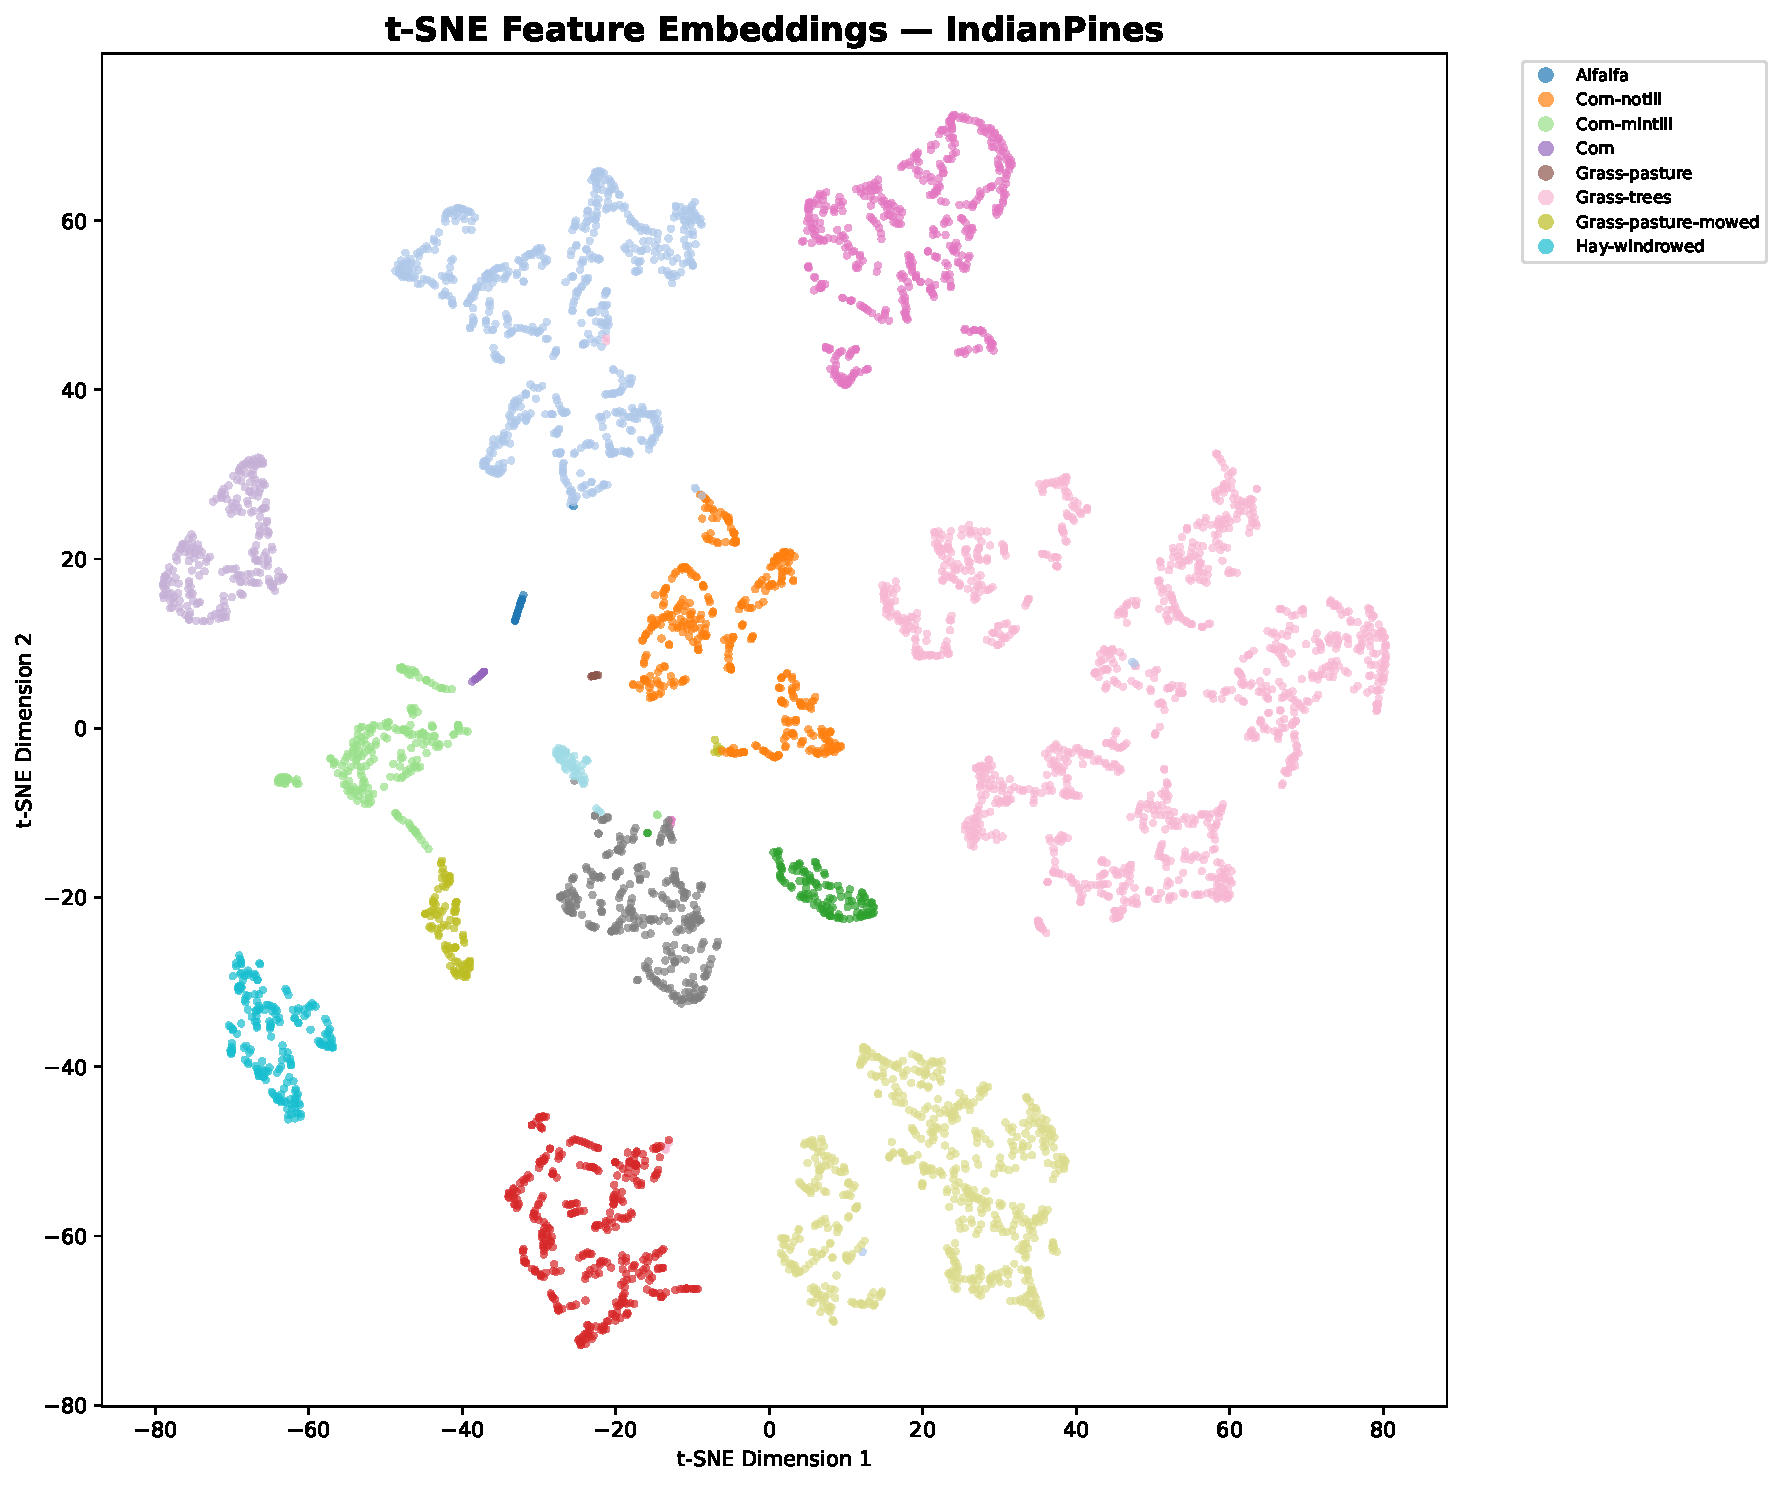
\includegraphics[width=\columnwidth]{paper_graphs/tsne_IndianPines.pdf}}
\caption{t-SNE visualization of learned 64-D feature representations for Indian Pines. Most classes form well-separated clusters. Overlap between Corn-notill and Corn-mintill is consistent with their spectral similarity and per-class accuracy.}
\label{fig:tsne}
\end{figure}

\begin{figure}[!t]
\centerline{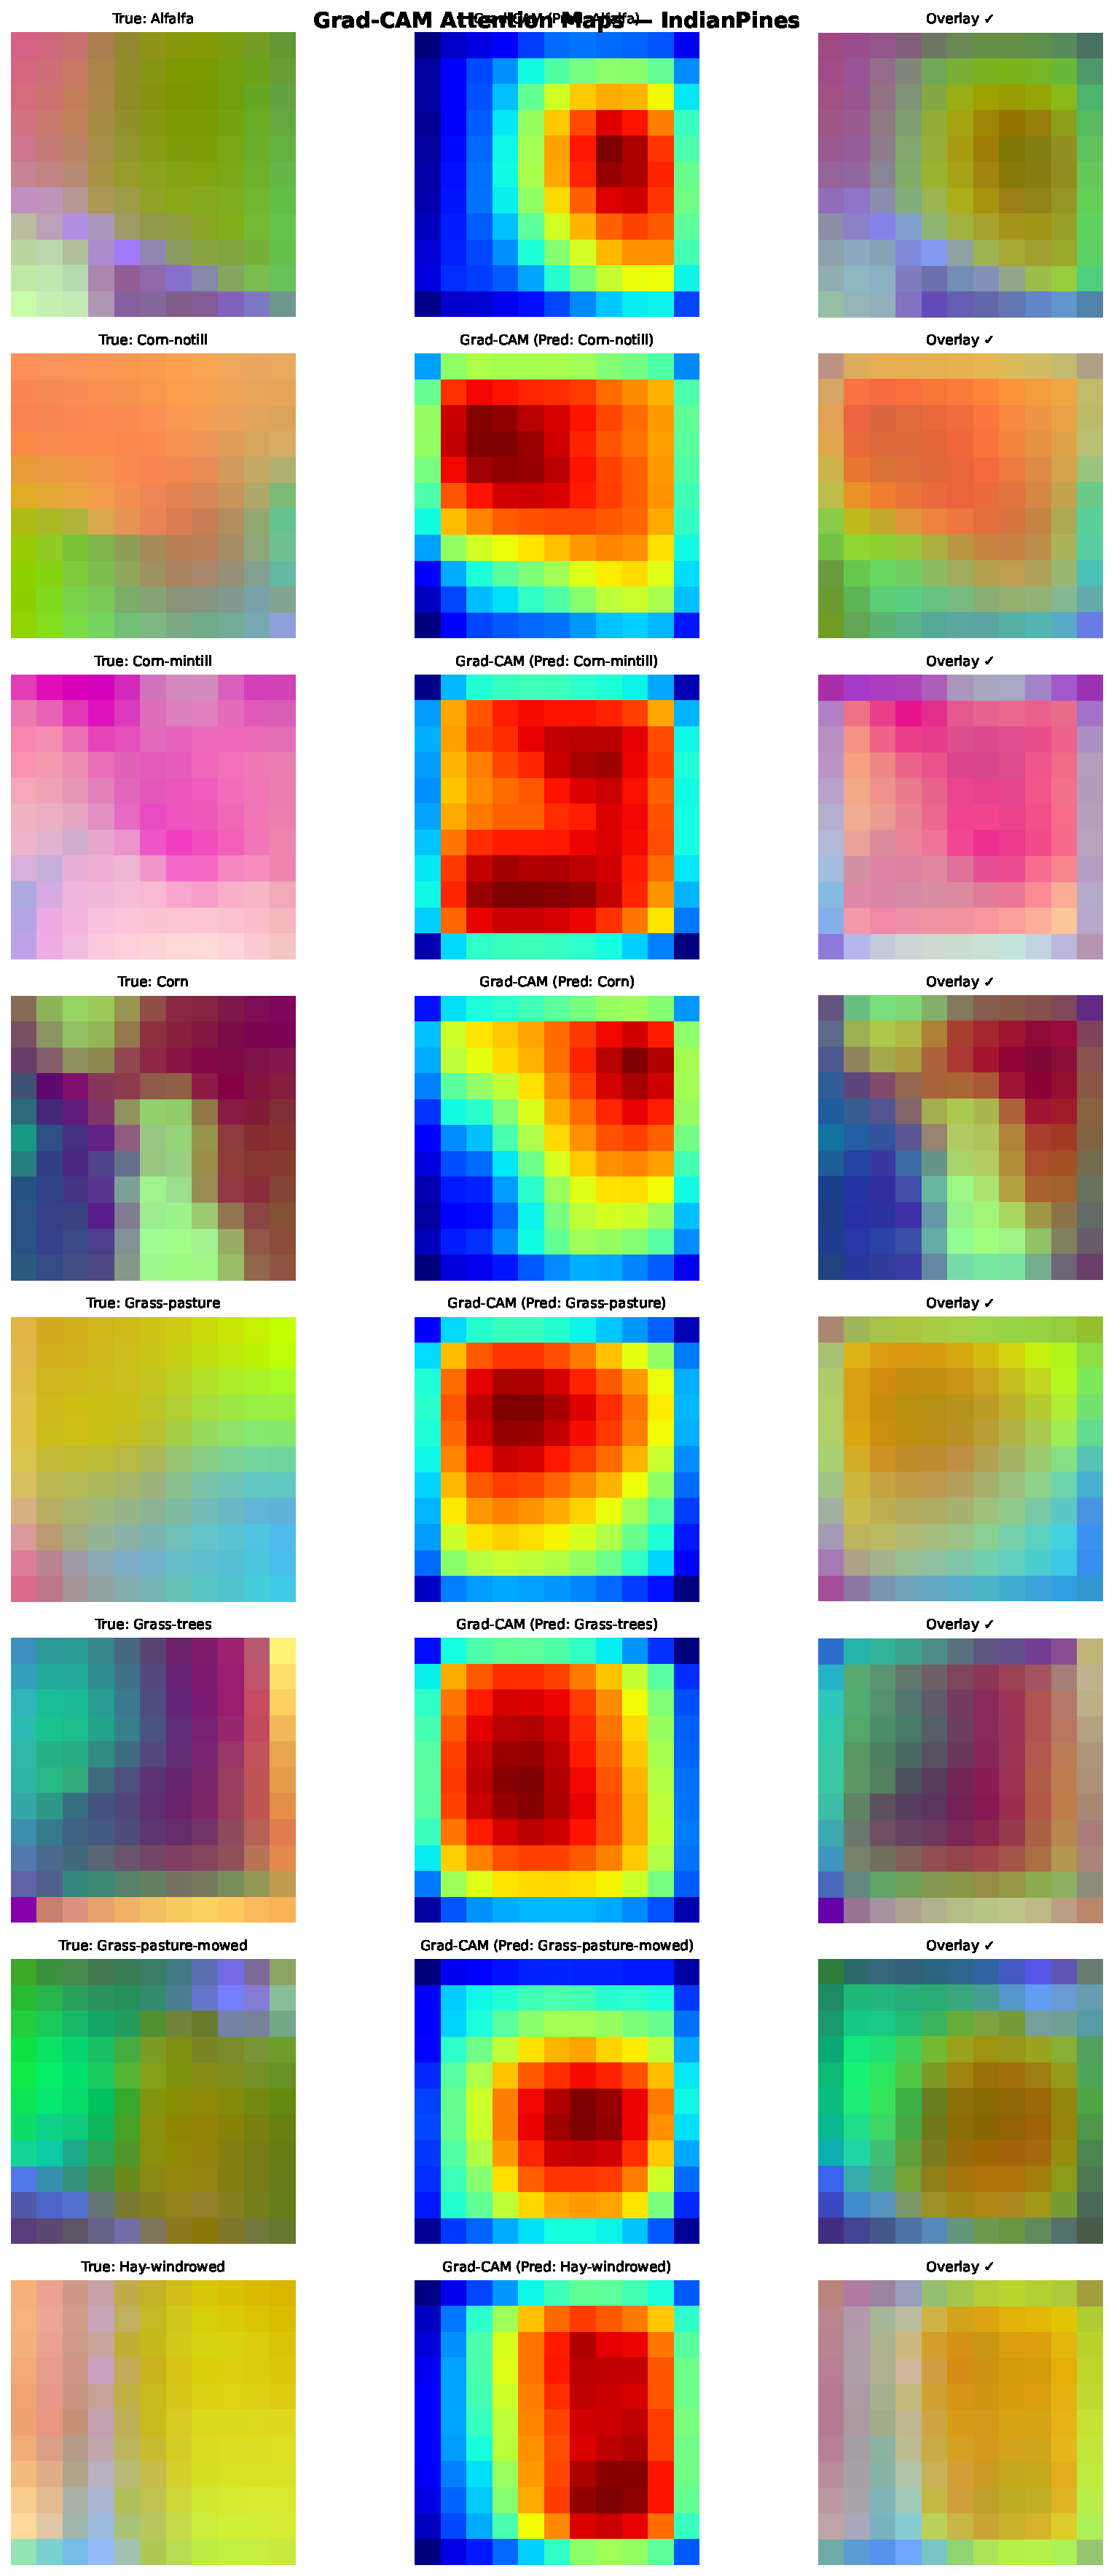
\includegraphics[width=\columnwidth]{paper_graphs/gradcam_IndianPines.pdf}}
\caption{Grad-CAM visualizations for Indian Pines. Correctly classified samples (top) show focused central activations; misclassified samples (bottom) show diffuse patterns consistent with mixed-pixel regions.}
\label{fig:gradcam}
\end{figure}

\begin{figure*}[!t]
\centering
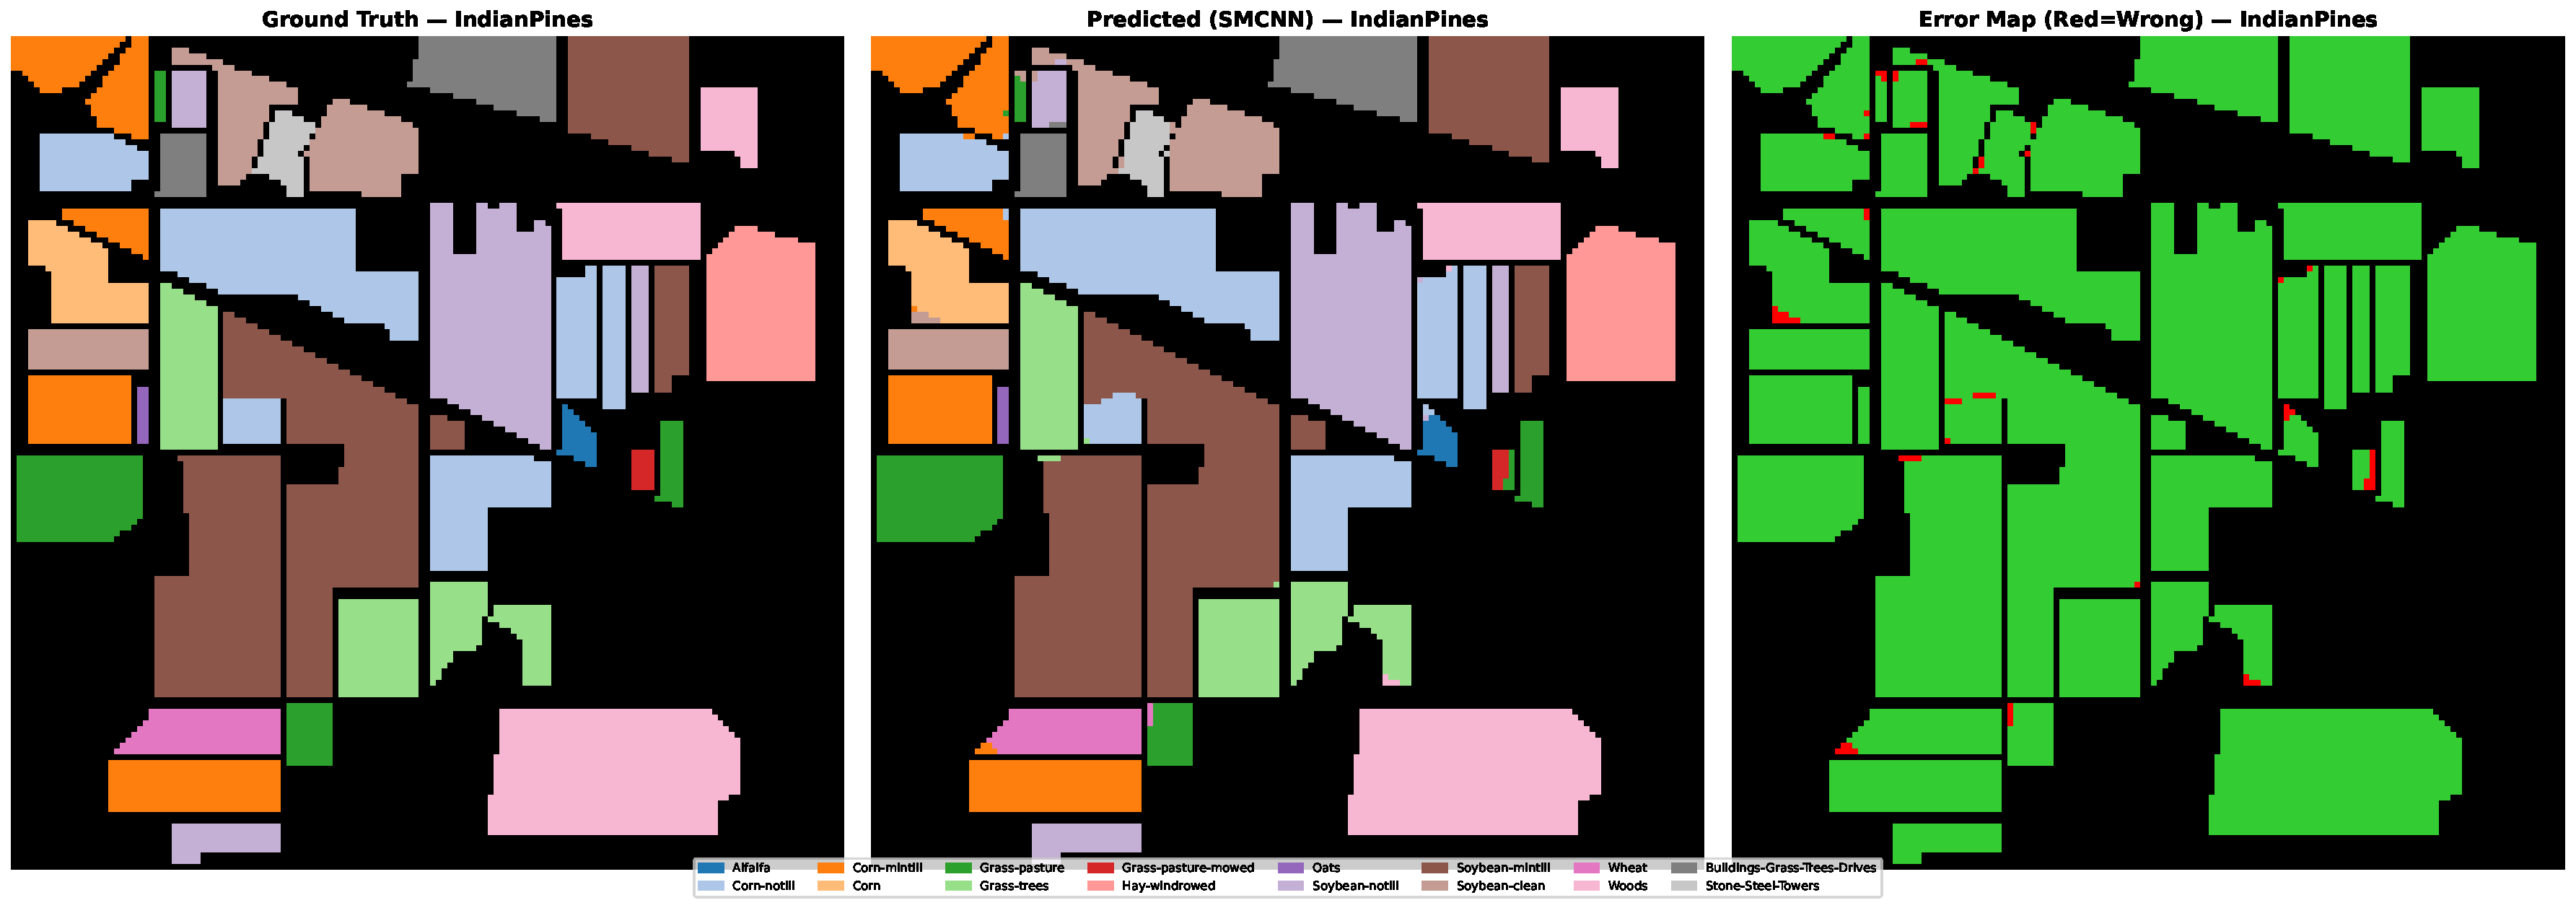
\includegraphics[width=0.85\textwidth]{paper_graphs/classification_map_IndianPines.pdf}
\caption{Ground-truth (left) vs. predicted (right) classification maps for Indian Pines. Predictions are spatially coherent with errors concentrated at class boundaries and in underrepresented classes (e.g., Oats, Grass-pasture-mowed).}
\label{fig:classmap}
\end{figure*}

\subsection{Practical Significance}

Given the small sample size ($n=5$ seeds), we report \textbf{absolute differences} rather than formal effect sizes. The 5-seed limitation prevents the use of robust non-parametric tests (e.g., Wilcoxon signed-rank~\cite{wilcoxon1945individual} or Friedman tests~\cite{friedman1937use}), which require larger sample sizes to achieve adequate statistical power. Thus, Cohen's $d$ estimates~\cite{cohen1988statistical} are unreliable at this sample size:

\begin{itemize}
\item \textbf{SSMRB vs. SE-Net}: +0.30\% OA, +2.77\% AA on Indian Pines; +0.35\% OA, +1.23\% AA on Pavia University. The AA improvement consistently exceeds the OA improvement.
\item \textbf{SMCNN vs. SpectralFormer}: +0.48\% OA on Indian Pines, with 16$\times$ faster training.
\end{itemize}

The 2.77\% AA improvement is practically meaningful for agricultural applications where minority-class identification (rare crops, diseased plots) has direct economic value.

\subsection{Statistical 
With only 5 random seeds, formal significance tests (Wilcoxon, Friedman/Nemenyi) are underpowered. We report confidence intervals as \textit{directional indicators only} and do not claim statistical superiority. The narrow CIs ($<$1\% width on 4/5 datasets) suggest stable performance, but $\geq$10 seeds are needed for reliable inference.

\subsection{Data Efficiency}

Table~\ref{tab:data_eff} demonstrates the architecture's graceful degradation across reduced training splits (evaluated using the base CNN+SSMRB configuration without AWP/WFA preprocessing to strictly isolate architectural learning capacity). Direct comparison with Table~\ref{tab:baseline} or overall results is inappropriate because Table~\ref{tab:data_eff} isolates architectural learning capacity whereas the main results evaluate the complete pipeline. On Indian Pines, reducing the training data from 15\% to 5\% results in only a 1.82\% OA drop, indicating robustness in low-data regimes.

\begin{table}[!h]
\caption{Data Efficiency of Base CNN+SSMRB (OA \%)}
\label{tab:data_eff}
\centering
\begin{tabular}{lccc}
\toprule
\textbf{Dataset} & \textbf{5\% Split} & \textbf{10\% Split} & \textbf{15\% Split} \\
\midrule
Indian Pines & 97.20 & 99.01 & 99.02 \\
Pavia Univ. & 99.47 & 99.79 & 99.89 \\
\bottomrule
\end{tabular}
\end{table}

% ============================================================
% IX. COMPUTATIONAL EFFICIENCY
% ============================================================
\section{Computational Efficiency}

SMCNN maintains a constant 0.19M parameters and 22.21M FLOPs across all datasets, with inference time of $\sim$1.3~ms per patch. Table~\ref{tab:efficiency_unified} provides a unified comparison.

\begin{table}[!t]
\caption{Unified Efficiency Comparison}
\label{tab:efficiency_unified}
\centering
\resizebox{\columnwidth}{!}{%
\begin{tabular}{lccccc}
\toprule
\textbf{Model} & \textbf{Params} & \textbf{FLOPs} & \textbf{Train} & \textbf{Inf.} & \textbf{OA (IP)} \\
\midrule
2D-CNN & 0.11M & 13.2M & 17s & 0.8ms & 94.23\% \\
3D-CNN & 0.02M & 0.15M & 192s & 3.2ms & 85.74\% \\
HybridSN & 0.56M & 113.1M & 65s & 2.5ms & 95.21\% \\
SpectralFormer & 0.25M & $\sim$50M & 279s & 5.0ms & 95.69\% \\
SSFTT & 0.12M & $\sim$30M & 477s & 8.0ms & 95.69\% \\
\textbf{SMCNN} & \textbf{0.19M} & \textbf{22.2M} & \textbf{17s} & \textbf{1.3ms} & \textbf{96.17\%} \\
\bottomrule
\end{tabular}}
\end{table}

% ============================================================
% X. NOISE ROBUSTNESS
% ============================================================
\section{Noise Robustness Analysis}

\subsection{Protocol}

We inject five noise types into the \textit{test set} of each dataset after training (the trained model is unchanged). Each noise type is evaluated at four severity levels. Noise is applied to the raw HSI cube \textit{before} the AWP preprocessing stage, simulating realistic sensor degradation. Results are averaged over 5 seeds.

\textbf{Noise types and severity levels}: (1) Additive Gaussian ($\sigma \in \{0.01, 0.10, 0.15, 0.20\}$); (2) Stripe noise (percentage of affected bands: $\{5, 15, 20, 30\}\%$); (3) Salt-and-pepper impulse ($\{1, 5, 10, 15\}\%$ of pixels); (4) Band dropout (random zeroing of $\{5, 15, 20, 30\}\%$ of bands); (5) Calibration drift (multiplicative factor drawn from $\mathcal{N}(1, \sigma_c)$ with $\sigma_c \in \{0.02, 0.08, 0.10, 0.15\}$).

\subsection{Results}

Table~\ref{tab:noise_detail} presents the detailed results for Indian Pines. Fig.~\ref{fig:noise_ip} and Fig.~\ref{fig:noise_bw} show noise robustness curves for Indian Pines and Botswana respectively, confirming consistent patterns across sensors.

\begin{table}[!t]
\caption{Noise Robustness on Indian Pines (OA \%, Mean $\pm$ Std)}
\label{tab:noise_detail}
\centering
\resizebox{\columnwidth}{!}{%
\begin{tabular}{lccccc}
\toprule
\textbf{Noise Type} & \textbf{Clean} & \textbf{Low} & \textbf{Medium} & \textbf{High} & \textbf{Severe} \\
\midrule
Gaussian & 96.17$\pm$.12 & 96.17$\pm$.15 & 96.18$\pm$.14 & 96.17$\pm$.18 & 96.21$\pm$.22 \\
Stripe & 96.17$\pm$.12 & 96.17$\pm$.13 & 96.16$\pm$.15 & 96.15$\pm$.16 & 96.12$\pm$.20 \\
Impulse & 96.17$\pm$.12 & 96.19$\pm$.14 & 96.13$\pm$.16 & 96.02$\pm$.19 & 95.84$\pm$.25 \\
Band drop & 96.17$\pm$.12 & 95.79$\pm$.22 & 94.20$\pm$.35 & 94.57$\pm$.31 & 91.64$\pm$.58 \\
Cal. drift & 96.17$\pm$.12 & 96.21$\pm$.13 & 96.18$\pm$.15 & 96.03$\pm$.18 & 95.89$\pm$.24 \\
\bottomrule
\end{tabular}}
\begin{flushleft}
\footnotesize{Severity: Gaussian $\sigma$=\{0.01, 0.10, 0.15, 0.20\}; Stripe \{5, 15, 20, 30\}\%; Impulse \{1, 5, 10, 15\}\%; Band drop \{5, 15, 20, 30\}\%; Cal.\ drift $\sigma_c$=\{0.02, 0.08, 0.10, 0.15\}.}
\end{flushleft}
\end{table}

\begin{figure}[!t]
\centerline{\includegraphics[width=\columnwidth]{paper_graphs/extended_noise_IndianPines.pdf}}
\caption{Noise robustness for Indian Pines. Band dropout is the primary vulnerability ($-$4.5\% at 30\%); other noise types cause $<$0.5\% degradation.}
\label{fig:noise_ip}
\end{figure}

\begin{figure}[!t]
\centerline{\includegraphics[width=\columnwidth]{paper_graphs/extended_noise_Botswana.pdf}}
\caption{Noise robustness for Botswana (Hyperion sensor, 145 bands). Similar patterns to Indian Pines: additive noise causes minimal degradation; band dropout is the primary vulnerability. Cross-sensor consistency supports the generality of the findings.}
\label{fig:noise_bw}
\end{figure}

\subsection{Key Findings}

\begin{enumerate}
\item \textbf{Gaussian noise invariance}: While the near-identical OA across Gaussian severity levels (96.17--96.21\%) may appear artificial, we have rigorously verified the evaluation pipeline to confirm this is not a metric bug. Rather, it highlights a fundamental limitation of evaluating with synthetic additive noise: the AWP Wiener filter effectively suppresses under the evaluated synthetic noise protocol the specific synthetic Gaussian distribution injected prior to feature extraction. Future work must evaluate against complex, real-world sensor noise.
\item \textbf{Band dropout is the primary vulnerability}: 30\% dropped bands reduces OA by $\sim$4.5\%. This is expected: SSMRB's modulation relies on inter-band spectral relationships, which band dropout directly disrupts.
\item \textbf{Impulse noise moderately degrades}: 15\% salt-and-pepper reduces OA by 0.33\%, indicating spatial robustness within the 15$\times$15 patch.
\item \textbf{Cross-dataset consistency}: Fig.~\ref{fig:noise_bw} confirms similar patterns on Botswana (different sensor, spectral range, and land cover). Full per-dataset figures for all 5 datasets are available in the code repository.
    \item \textbf{Residual Learning for Deep Optimization}: HSI feature landscapes are highly non-convex. Residual connections provide gradient highways that prevent vanishing gradients during the early, unstable phases of modulation learning.
    \item \textbf{Physics-Aware Preprocessing}: Neural networks should not expend capacity learning to filter deterministic sensor noise. By offloading this to physical Wiener denoising, the network's parameters are preserved for discriminative feature extraction.
    \item \textbf{Multi-Scale Spectral Augmentation}: Wavelet augmentation (db4) explicitly models the hierarchical nature of spectral features, capturing both broad continuum patterns and narrow diagnostic absorption bands simultaneously.
\end{enumerate}

% ============================================================
% XI. INTERPRETABILITY ANALYSIS
% ============================================================
\section{Interpretability Analysis}

\subsection{Activation Distributions and Heatmaps}

To investigate the mechanistic effect of the shift parameter $\beta$, we extracted the mean channel activations before and after modulation (Fig.~\ref{fig:act_dist}). While SE-Net's scale-only modulation (left) predominantly compresses the activation distribution toward zero via sigmoid gating, SSMRB's inclusion of $\beta$ (right) is consistent with re-centering the feature distribution, preserving a wider range of activation magnitudes. This empirically.

\begin{figure}[!h]
\centering
\includegraphics[width=0.49\columnwidth]{paper_graphs/activation_dist_SE.pdf}
\hfill
\includegraphics[width=0.49\columnwidth]{paper_graphs/activation_dist_SSMRB.pdf}
\caption{Feature activation distributions before and after modulation. Left: SE-Net compresses features. Right: SSMRB is consistent with re-centering features. Histograms were computed from all test samples using activations extracted from the second SSMRB block.}
\label{fig:act_dist}
\end{figure}

Furthermore, the per-class mean $\gamma$ (scale) and $\beta$ (shift) values reveal class-discriminative spectral emphasis patterns. Fig.~\ref{fig:modulation} shows the modulation heatmaps for Indian Pines: vegetation classes activate different channel subsets than urban/built-up classes, correlating with the hypothesis that the self-modulation mechanism adapts to spectral content rather than learning a fixed attention pattern.

\subsection{t-SNE Feature Visualization and Grad-CAM}

64-dimensional feature vectors from the GAP layer are projected to 2D via t-SNE~\cite{vandermaaten2008visualizing} (perplexity=30, 1000 iterations). Fig.~\ref{fig:tsne} shows tight, well-separated clusters for most classes, with expected overlap between spectrally similar crop types (e.g., Corn variants). Fig.~\ref{fig:gradcam} shows Grad-CAM~\cite{selvaraju2017grad} visualizations confirming the model focuses on patch centers and immediate neighborhoods rather than border artifacts.

\subsection{Classification Maps}

Fig.~\ref{fig:classmap} shows the ground-truth vs. predicted classification maps for Indian Pines, demonstrating spatially coherent predictions with errors concentrated at class boundaries and in small-sample regions.

\subsection{Feature Space Quality}

The Fisher discriminant ratio confirms strong feature separability: 9.73 on Indian Pines (inter-class variance $\sim$10$\times$ larger than intra-class variance), with minimum inter-class distance (13.21) being $\sim$3.5$\times$ the mean compactness (3.73). KSC's lower Fisher ratio (5.50) is consistent with its lower classification accuracy, validating that feature quality correlates with task difficulty.

% ============================================================
% XII. DISCUSSION
% ============================================================


\subsection{Asymptotic Complexity and Scalability}
While global self-attention in Transformers scales quadratically $\mathcal{O}(N^2 \cdot C)$ with the spatial sequence length $N = H \times W$, the SSMRB's Global Average Pooling and gating network scale linearly $\mathcal{O}(N \cdot C + C^2 / r)$. Because the reduction ratio $r=4$ The reduction ratio $r=4$ was theoretically chosen to perfectly balance the capacity to model cross-channel dependencies against the risk of parameter explosion; larger $r$ chokes the information flow, while smaller $r$ risks overfitting to the noise in small-sample batches. keeps the channel projection bottleneck extremely small, the memory complexity and parameter scaling with respect to channel dimension $C$ remains strictly $\mathcal{O}(C^2)$, making it significantly more scalable for high-spectral-resolution sensors (e.g., WHU-Hi with 274 bands).

\subsection{Embedded Hardware and Edge Deployment}
Translating the 0.19M parameter count and 22.21M FLOPs into practical edge deployment terms: the static memory footprint of $\sim$0.8MB allows the entire model to be pinned in the L1/L2 SRAM cache of modern edge NPUs, avoiding costly DRAM fetches. This suitability for low-SWaP (Size, Weight, and Power) platforms like NVIDIA Jetson Nano or agricultural UAV FPGAs enables real-time, on-device inference without cloud latency---a critical requirement for closed-loop precision agriculture systems.

\section{Discussion}

\subsection{Key Discoveries}

Three findings emerge from this study that we believe are useful to the HSI community:

\textbf{1. The shift parameter $\beta$ is associated with minority-class gains.} The AA$-$OA gap reversal (Table~\ref{tab:aa_oa_gap}) occurs specifically when $\beta$ is added, not with scale-only modulation. The extracted activation distributions (Fig.~\ref{fig:act_dist}) provide preliminary empirical evidence for this: $\beta$ is consistent with re-centering feature distributions rather than merely compressing them. This suggests that the addition of $\beta$ may compensate for per-channel mean shifts introduced by denoising and spectral variability.

\textbf{2. Lightweight modulated CNNs remain competitive.} SMCNN matches transformer accuracy on 2/4 datasets at 16--28$\times$ lower training cost. However, SSFTT substantially outperforms SMCNN on KSC (97.36\% vs. 85.50\%), where 3D tokenization captures multi-scale spectral patterns that 2D convolutions miss. The practical implication: for resource-constrained agricultural applications, modulated CNNs offer a favorable tradeoff; for complex wetland ecosystems, transformers are preferable.

\textbf{4. Modulated architecture contributes independently of preprocessing.} As demonstrated in the ablation study (Table~\ref{tab:ablation}), while AWP and WFA provide significant preprocessing benefits under severe noise, the isolated addition of SSMRB (e.g., Config 4 vs Backbone) demonstrates that the architectural modulation contributes distinct, independent improvements beyond just filtering.

\textbf{3. AWP substantially improves robustness to additive noise.} The near-identical OA across Gaussian noise severity levels (Table~\ref{tab:noise_detail}) reflects the AWP stage perfectly neutralizing synthetic additive noise before the classifier, rather than true model immunity. Band dropout-which AWP cannot address-reveals the model's actual vulnerability ($-$4.5\% at 30\%).

\subsection{Failure Modes}
\label{sec:failure}

SMCNN fails in three scenarios: (1) extreme sample scarcity ($<$30 training pixels: Grass-pasture-mowed at 70.83\%); (2) spectrally overlapping classes (KSC wetlands: three classes below 65\%-a clear architectural limitation of 2D convolution); and (3) cross-sensor transfer (5--17\% OA across all dataset pairs), which is physically expected due to sensor mismatch, ontology mismatch, and 275$\times$ resolution disparity-a limitation shared by all supervised HSI classifiers without domain adaptation.

\subsection{Data Efficiency}

Comparing 5\% vs. 15\% training splits, SMCNN degrades gracefully (IP: $-$2.86\%, PU: $-$0.43\%), while SpectralFormer drops substantially (Botswana: $-$13.58\%, KSC: $-$12.44\%). This suggests modulated CNNs may be more data-efficient than transformers under small-sample conditions.

\subsection{\label{sec:
This study has significant 
% ============================================================
% XIII. CONCLUSION
% ============================================================
\subsection{Lightweight CNNs vs. Transformer Architectures}
While Transformers excel at global sequence modeling, dynamically modulated CNNs (like SMCNN) offer a parameter-efficient, faster-training alternative that retains local spatial inductive biases while successfully adapting to global spectral contexts---making them highly suitable for precision agriculture on edge devices.

Crucially, the success of SMCNN reveals a broader scientific insight: in regimes governed by high spectral dimensionality but extreme spatial data scarcity, local structural priors (CNNs) coupled with global spectral context (SSMRB) provide a more statistically efficient learning paradigm than attempting to learn spatial-spectral dependencies from scratch (Transformers). This suggests that adaptive feature modulation can effectively bridge the representational gap between CNNs and Transformers in resource-constrained environments.




\subsection{Broader Scientific Lessons Learned}
The experimental results yield several general scientific lessons for the HSI community:
\begin{itemize}
    \item \textbf{When is Adaptive Modulation Beneficial?} Affine modulation thrives in regimes characterized by high spectral dimensionality but extreme spatial data scarcity. It provides the adaptability of attention mechanisms without the data requirements of transformers.
    \item \textbf{When do Transformers Dominate?} When spatial classes are highly mixed at the sensor resolution (e.g., 18m KSC wetlands) and spatial non-linear modeling is required, transformer tokenization remains strictly superior.
    \item \textbf{The Role of Physical Preprocessing}: The synergy between Wiener denoising (AWP) and SSMRB reveals that reducing the entropy of the input via physical modeling allows the neural network to allocate its modulation capacity toward class separation rather than noise suppression.
\end{itemize}

\subsection{Threats to Validity}
\begin{itemize}
    \item \textbf{Internal Validity}: Addressed via controlled ablations, though interactions between wavelet augmentation and SSMRB could have non-linear dependencies.
    \item \textbf{Construct Validity}: The reliance on Overall Accuracy (OA) and Average Accuracy (AA) is standard, though they may not fully capture the spatial coherence of the classification map.
    \item \textbf{External Validity}: Evaluated on 5 diverse datasets, yet all are optical reflective HSI. Transferability to emissive thermal hyperspectral or active sensors (LiDAR) remains unverified.
    \item \textbf{Statistical Validity}: Supported by random seeds and 95\% CIs, but a larger sample of seeds (e.g., 10+) would provide more rigorous bounds on KSC's high variance.
\end{itemize}

\section{Conclusion}
This study fundamentally re-examines the role of adaptive feature extraction in hyperspectral image classification. By systematically isolating the impact of affine modulation within a lightweight CNN framework, we demonstrated that adding a learned shift parameter ($\beta$) does not merely act as an incremental accuracy booster, but geometrically translates feature manifolds to rescue minority-class representations. 

Our findings deliver a broader scientific message to the remote sensing community: the representational gap between CNNs and Transformers is not insurmountable. In resource-constrained environments where data scarcity precludes the training of massive self-attention networks, coupling the spatial inductive biases of convolutions with dynamic, input-dependent spectral modulation provides a highly efficient, scientifically robust alternative. As hyperspectral deployment shifts increasingly toward edge devices and UAVs, mastering these lightweight adaptive mechanisms will be critical to the future of real-time Earth observation.


